\documentclass[a4paper,11pt,final]{article}
% Pour une impression recto verso, utilisez plutôt ce documentclass :
%\documentclass[a4paper,11pt,twoside,final]{article}

\usepackage[left=2cm,right=2cm,top=2cm,bottom=2cm]{geometry}
\usepackage[english,francais]{babel}
\usepackage[utf8]{inputenc}
\usepackage[T1]{fontenc}
\usepackage[pdftex]{graphicx}
\usepackage{setspace}
\usepackage{hyperref}
\usepackage[french]{varioref}

\newcommand{\reporttitle}{Movie Manager}     % Titre
\newcommand{\reportauthor}{Vincent \textsc{ALBERT}} % Auteur
\newcommand{\reportsubject}{Rapport de projet SD} % Sujet
\newcommand{\HRule}{\rule{\linewidth}{0.5mm}}
\setlength{\parskip}{1ex} % Espace entre les paragraphes

\begin{document}
  \begin{titlepage}

\begin{center}

\begin{minipage}[t]{0.48\textwidth}
  \begin{flushleft}
	
\includegraphics [width=50mm]{images/logo-telecom.png} \\[0.5cm]
      \textsc{\LARGE Telecom Nancy}
  \end{flushleft}
\end{minipage}
\begin{minipage}[t]{0.48\textwidth}
  \begin{flushright}
    
\includegraphics [width=50mm]{images/logo-ul.jpg} \\[0.5cm]
    \textsc{\LARGE Université de Lorraine}
  \end{flushright}
\end{minipage} \\[1.5cm]


	\textsc{\Large \reportsubject}\\[0.5cm]
	\HRule \\[0.4cm]
	{\huge \bfseries \reporttitle}\\[0.4cm]
	\HRule \\[1.5cm]
	
	\begin{minipage}[t]{0.3\textwidth}
 	 	\begin{flushleft} \large
  		\end{flushleft}
	\end{minipage}
	\begin{minipage}[t]{0.6\textwidth}
  		\begin{flushright} \large
    		\emph{Auteurs :} \\
    		Nicolas \textsc{Bédrine} \\
    		Vincent \textsc{Albert} \\
  		\end{flushright}
	\end{minipage}

\vfill

{\large \today{}}

\end{center}

\end{titlepage}

  \cleardoublepage % Dans le cas du recto verso, ajoute une page blanche si besoin
  \renewcommand\thepage{}
  \tableofcontents % Table des matières
  \sloppy          % Justification moins stricte : des mots ne dépasseront pas des paragraphes
  \cleardoublepage
  \renewcommand\thepage{\arabic{page}}
  \setcounter{page}{1}
  
  \section{Présentation du sujet} % Pas de numérotation
\addcontentsline{toc}{section}{Présentation du sujet} % Ajout dans la table des matières

\subsection{Un rapide résumé}
Le logiciel MovieManager est un gestionnaire de films permettant de gérer les films vus par l'utilisateur, de charger une base de films à partir d'un fichier texte, de les exporter en format json, et de créer une liste de propositions de films à voir.

\begin{figure}[!ht]
    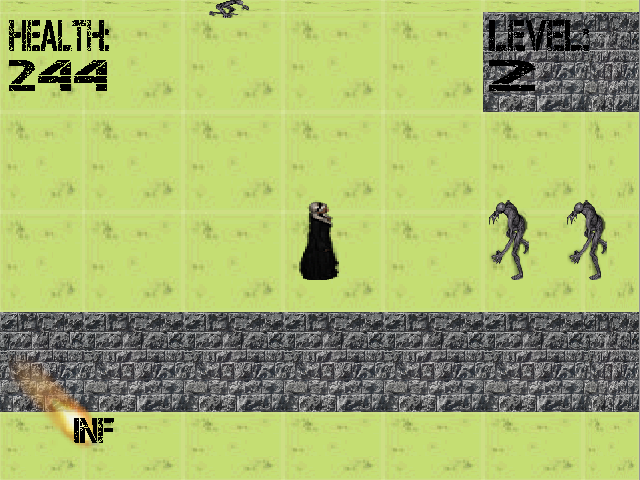
\includegraphics[width=0.5\textwidth]{./images/snapshot1.png}
    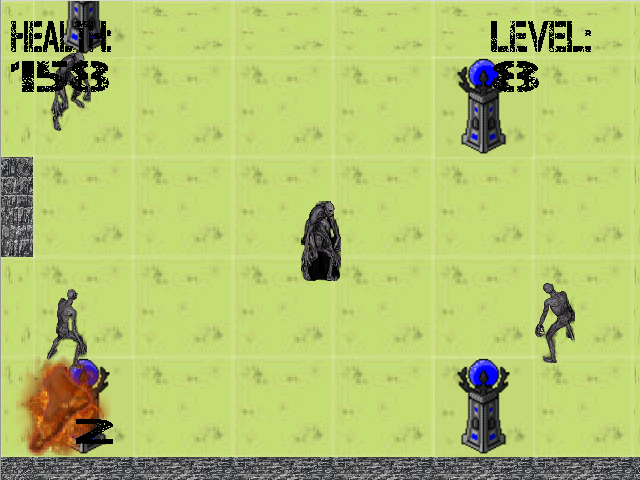
\includegraphics[width=0.5\textwidth]{./images/snapshot2.png}
    \caption{Captures d'écran}
\end{figure}

Nous n'avons pas inclus de vue en console, mais uniquement une vue graphique. En effet, après demande de renseignements, on nous a dit qu'il n'était pas nécessaire de l'implémenter.

\subsection{Les objectifs recherchés}
Le but du programme est d'établir un standard de films qui correspond aux goûts de l'utilisateur. Une fois ce standard défini, nous recherchons dans le modèle les films qui lui sont proches. Ainsi, on ne proposera pas forcément les suites de films déjà vus par l'utilisateur si lesdits films ne font pas partie de ses films les plus regardés. \\
Dans le calcul de la distance entre les films, toutes les composantes sont prises en compte. On leur attribue des poids définis arbitrairement. Ainsi, voici leur hiérarchie :

\begin{itemize}
	\item Titre du film
	\item Liste des genres
	\item Réalisateur
	\item Liste des acteurs
	\item Type (Film ou série TV)
\end{itemize}


  \cleardoublepage
  \section{Organisation}
\subsection{Les outils utilisés}

\subsection{UML du modèle}



  \cleardoublepage
  \section{La phase de développement}

\subsection{Répartition des tâches}

\begin{itemize}
\item[•]{Conception}

	\begin{itemize}
		\item{Nicolas : 3h}
		\item{Vincent : 3h}
	\end{itemize}

\item[•]{Codage}

	\begin{itemize}
		\item{Nicolas : 12h}
		\item{Vincent : 15h}
	\end{itemize}

\item[•]{Tests}

	\begin{itemize}
		\item{Nicolas : 4h}
		\item{Vincent : 2h}
	\end{itemize}

\item[•]{Rédaction du rapport}
	\begin{itemize}
		\item{Nicolas : 1h}
		\item{Vincent : 2h}
	\end{itemize}
\end{itemize}

\subsection{Les problèmes rencontrés}

La partie graphique n'a pas posé de problèmes particuliers étant donné l'utilisation de la bibliothèque swing. Nous avons respecté le pattern MVC en faisant hériter les ListMovie de la classe AbstractTableModel. \\
Cependant, le modèle n'a pas été aussi généreux. En effet, nous avons voulu implémenter l'algorithme HMeans vu en cours de mathématiques numériques pour la classification des données. Nous avons eu en effet beaucoup de mal. \\
Nous avons aussi rencontrés des problèmes dont nous n'avons pas réussi à cibler l'origine ; nous avons pu alors appréhender une nouvelle fonctionnalité de git, à savoir git reset qui nous a permis de revenir à un commit précédent.
  \cleardoublepage
  
  \thispagestyle{empty}
\end{document}

